\documentclass[a4paper,10pt]{article}

\usepackage[utf8]{inputenc} 
\usepackage[T1]{fontenc}     
\usepackage[francais]{babel}

\usepackage[top=2cm, bottom=2cm, left=2cm, right=2cm]{geometry}

\usepackage{graphicx}

\usepackage{amsthm}
\usepackage{amsmath}
\usepackage{amssymb} 	

\usepackage{url}

\usepackage{algorithm}
\usepackage{algorithmic}
%\usepackage[backref, hidelinks]{hyperref}

\usepackage{a4wide}

%%%% debut macro %%%%
\newenvironment{changemargin}[3]{\begin{list}{}{%
\setlength{\topsep}{0pt}%
\setlength{\leftmargin}{0pt}%
\setlength{\rightmargin}{0pt}%
\setlength{\topmargin}{0pt}%
\setlength{\listparindent}{\parindent}%
\setlength{\itemindent}{\parindent}%
\setlength{\parsep}{0pt plus 1pt}%
\addtolength{\leftmargin}{#1}%
\addtolength{\rightmargin}{#2}%
\addtolength{\topmargin}{#3}%
}\item }{\end{list}}
%%%% fin macro %%%%

\newcommand{\argmax}[1]{\underset{#1}{\operatorname{argmax}}\;}

\title{Thompson Sampling (PSRL) under bias span constraint}
\author{Pierre \textsc{Bizeul}, Jules \textsc{Kozolinsky} }
\date\today 
\makeindex

\begin{document}

\maketitle
\tableofcontents

\section{Goal of project}
The Exploration-Exploitation trade-off is a fundamental dilemma in on-line reinforcement learning. Algorithms addressing this dilemma with theoretical performance guarantees have been proposed for the discounted, average and finite horizon settings. In the finite horizon setting, the usual criterion of performance is the notion of “regret” as in MAB. One of the current state-of-the-art algorithms PSRL \cite{osband2013more}  has a regret scaling linearly with the “diameter” of the unknown MDP in the worst-case (the diameter being a measure of how easy it is to navigate between any two states of the MDP). Although it has been shown that the dependency in the diameter is unavoidable in the worst-case, when additional properties on the optimal policy are known beforehand, the regret can, in theory, be drastically improved \cite{bartlett2009regal}. Unfortunately, exploiting this additional prior knowledge on the optimal policy requires solving an optimization problem (namely, “planning under bias span constraint”) and no algorithm has been derived so far to solve it. We recently started investigating a new Bellman operator converging to the solution of this problem for many MDPs. In this research project, the student(s) is/are expected to:
\begin{enumerate}
\item  Implement PSRL,
\item  Integrate the modified Bellman operator to PSRL,
\item Compare the empirical regret of the two.
\end{enumerate}

\section{Introduction}
\subsection{Notations}
\paragraph{Policy\\}
A policy $\pi$ is defined as $\pi: X \rightarrow A$.
\paragraph{Long-term average reward\\}
Long-term average reward $\rho_{\pi}(M)$ of a policy $\pi$ is defined as : 
\begin{align*}
\rho_{\pi}(M) = \lim\limits_{T \rightarrow \infty} \dfrac{1}{T}E(T) = \lim\limits_{T \rightarrow \infty} \dfrac{1}{T}\sum\limits_{t = 1}^{T} r_t
\end{align*}
where $T$ is the number of time steps and 
$E(T)$ is the total expected reward after $T$ steps.

\paragraph{Optimal policy\\}
A policy is called \textit{optimal} if it maximizes the long-term average reward : 
\begin{align*}
\pi^{*}(M) =  \argmax{\pi} \rho_{\pi}(M)
\end{align*}
We note: $\rho^{*}(M) = \rho_{\pi^{*}(M)}(M)$.

\subsection{Exploration-exploitation dilemma}
Explore the environment to estimate its parameters vs Exploit the estimates to collect reward (See Figure \ref{regret}).

\begin{figure}[h]
	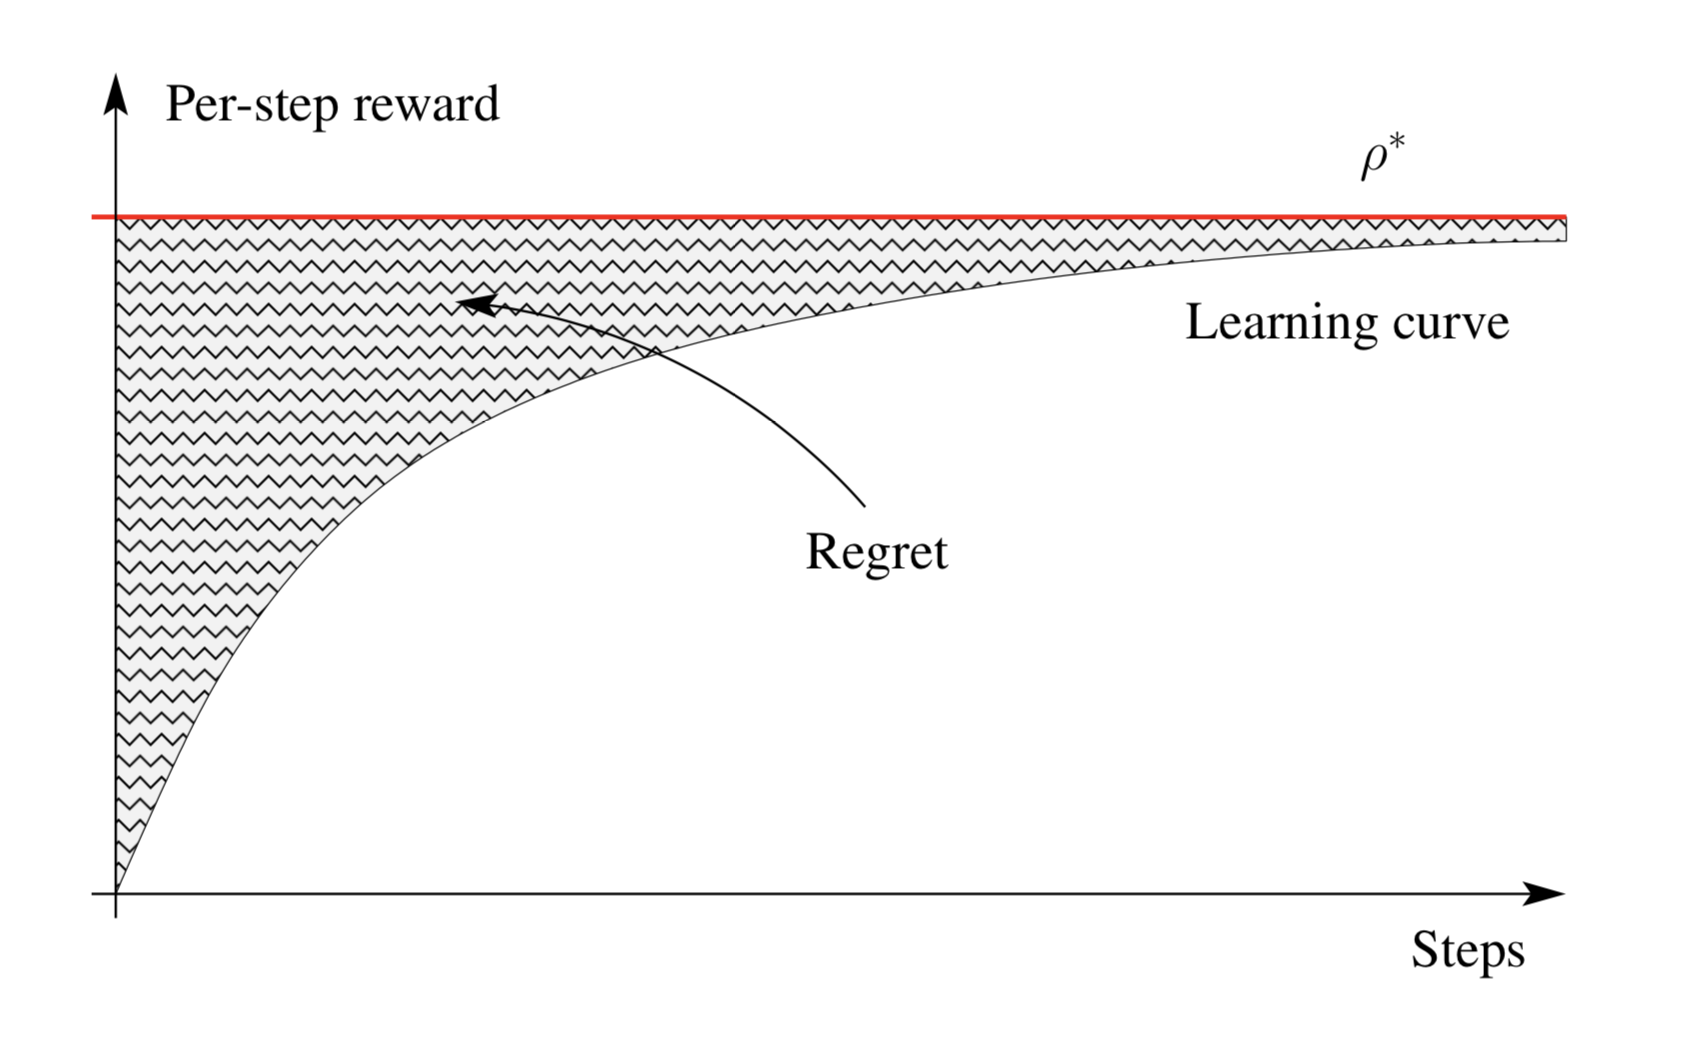
\includegraphics[width=\textwidth]{regret.png}
   \caption{Exploration-Exploitation in RL}
   \label{regret}
\end{figure}

\paragraph{Cumulative regret\\}
Cumulative regret $R_{\pi}(T)$ of a policy $\pi$ is defined as : 
\begin{align*}
R_{\pi}(T) = T\rho^{*} - \sum\limits_{t = 1}^{T} r_t
\end{align*}

\section{Upper-confidence Bound for RL}
\subsection{Upper-confidence bound}
\subsection{UCRL2 Algorithm}

\section{Thompson Sampling for RL}

\bibliographystyle{plain}
\bibliography{biblio}


\end{document}
